\documentclass[conference]{IEEEtran}
\usepackage{iftex}
\ifXeTeX
\usepackage{fontspec}
\setmainfont{Times New Roman}
\setsansfont{Arial}
\setmonofont{Courier New}
\else
\usepackage[T1]{fontenc}
\usepackage{mathptmx}
\usepackage{microtype}
\fi
\usepackage{amsmath,amssymb,array,url,graphicx,etoolbox,tikz}
\usetikzlibrary{positioning,arrows.meta}
\IfFileExists{booktabs.sty}{\usepackage{booktabs}}{\newcommand{\toprule}{\hline}\newcommand{\midrule}{\hline}\newcommand{\bottomrule}{\hline}}
\patchcmd{\abstract}{---}{: }{}{}
\patchcmd{\IEEEkeywords}{---}{: }{}{}
\newcolumntype{L}[1]{>{\raggedright\arraybackslash\hyphenpenalty=10000\exhyphenpenalty=10000}p{#1}}

% ======================================================================
% VALUES OF THE FINAL-BUILD DEMONSTRATION RUNS.
% Every macro in this block is a PLACEHOLDER until the runs on the final
% application build are recorded. Replace each \TBF{...} by the recorded
% value. \TBF prints a visible marker, so that an unfilled value cannot be
% read as a result. The comment after each macro shows the FORM of a value;
% the examples are not results.
% The sentences around these macros (Section VIII-C, "Runs on the final
% build") state the limits of those runs as fixed text. Read them again
% when the values are filled, and change them if the conditions differ
% (for example, if a person reviews a run, or if a route reaches a real
% model). The same holds for the last sentences of the abstract, for the
% route sentences of Section VII-D and for the conclusion.
% Keep the paper at 8 pages: with values of the lengths shown here, about
% nine text lines of the last column stay free.
% ======================================================================
\newcommand{\TBF}[1]{\textbf{[to fill: #1]}}
\newcommand{\PaperDate}{14 November 2026}
\newcommand{\FinalRunDate}{14 November 2026 (UTC)}
%   form: 14 November 2026 (UTC)
\newcommand{\FinalRevision}{\texttt{ff92666}}
%   form: \texttt{0a1b2c3}  (first seven characters of the revision)
\newcommand{\FinalFingerprint}{\texttt{22ba794e2091}}
%   form: \texttt{0123456789ab}
\newcommand{\FinalEvidencePath}{\texttt{docs/evidence/2026-11-14-integrated/}}
%   form: \url{docs/evidence/2026-11-14/}
\newcommand{\FinalModel}{Claude Opus (sub-agent alias of the session)}
%   form: claude-fable-5-2  (the name that the route declares; no other word)
\newcommand{\FinalScenarioItems}{ten}
%   form: ten  (a number word; the sentence continues "invented items")
\newcommand{\FinalManual}{10 eligible items; 7 after Apply; 10 after Undo}
%   form: 8 eligible items; 6 after Apply; 8 after Undo
\newcommand{\FinalTags}{Three category names and six tags approved (Cooking and its subcategories; among the tags, street food); 16 application checks passed; 10; 6; 10}
%   form: Category Food and tag street food approved; 10 eligible items; 6 after Apply; 10 after Undo
\newcommand{\FinalMixed}{Two controls proposed and applied with one approval (show more Music, remove the food terms); two items moved up; 10; 6; 10}
%   form: Two controls proposed and applied with one approval (boost Music, exclude Food); 10; 6; 10
\newcommand{\FinalAbstain}{Ambiguous: the model asked for a clarification. Daily limit: reported by the model as unsupported. Negated command: stopped by the rule before any call. No match: reported by the model. Nothing applied in the four cases}
%   form: Ambiguous: the model asked for a clarification. Negated: stopped by the rule before any call.
%         Unsupported and no match: reported by the model. Nothing applied in the four cases
\newcommand{\FinalDescriptions}{Second scenario: three items selected, each with a checked quotation; 8; 5; 8. Category-and-tag scenario: one item; 10; 9; 10}
%   form: Three items selected, each with a checked quotation; 8; 5; 8
\newcommand{\FinalNewCategory}{Label \emph{Damaged object repaired and kept in use}; 3 members; the two calls agreed on every item, so nothing was withheld for a disagreement; 8; 5; 8}
%   form: Label \emph{Edible food}; 3 members; 1 unknown; 8; 5; 8
\newcommand{\FinalFictional}{One draft approved and added to the separate list (1 item); removed (0 items); the feed stayed at 10}
%   form: One draft accepted and admitted to the separate feed (1 item); removed (0 items)
\newcommand{\FinalAssertions}{the three runs made 13 model calls, 321 of 321 scripted checks passed, and the AI operator made 19 review decisions, all approvals}
%   form: 212 of 212 scripted assertions passed, and the AI operator made 19 review decisions
%   (a clause without a final period; it completes the sentence "In total, ...")
\newcommand{\FinalRouteChecks}{the connection check and the route trial (nine bundled requests) ran through one stand-in program for the command-line route and one stand-in server for each of the two HTTP routes, with authored replies and no error}
%   form: the route trial ran the bundled requests through one stand-in program for the command-line
%         route and one stand-in server for each of the two HTTP routes
%   (a clause without a final period; it completes the sentence "Route checks: ...")
% One sentence that only the student can confirm. It prints a visible marker.
\newcommand{\StudentConfirm}[1]{#1 \textbf{[student to confirm]}}
% ======================================================================

\title{LLM-Mediated Natural Language Controls for Short-Video Recommender Systems: An Offline Study of Controllability}
\author{\IEEEauthorblockN{Vibhor Malik}\IEEEauthorblockA{M.Sc. in Applied Computing, British Columbia Institute of Technology\\COMP 9500 Research Project. Supervisor: Borna Noureddin. \PaperDate}}
\begin{document}
\bstctlcite{paperBSTcontrol}
\maketitle
\thispagestyle{plain}\pagestyle{plain}
\begin{abstract}
This offline study asks how much a deterministic category control changes the exposure of a short-video feed and what it costs in next-item ranking quality, how reliably a language model interprets a request, and whether control can go beyond fixed category identifiers. It separates interpretation by a model from a deterministic policy. In Experiment 1, target-category exposure is 79.2\% under a category policy against 11.6\% under one-item feedback, and hard exclusion gives zero muted exposure; the policy itself explains both effects. A local Llama model parses 79 of 100 requests, below the 85\% target, and NDCG@10 for boosts is 0.0164 against 0.0301. In Experiment 2, on 100 fresh synthetic requests with model-written references, Llama matches 76 references and a rule parser 11. Induced control success is 20.1\% against 3.8\% for item feedback, NDCG@10 is 0.0258 against 0.0318, and conditional requests never succeed. A reviewed workflow then implements control beyond category identifiers: a model proposes, the application checks schema and evidence, a reviewer approves or rejects, and one deterministic policy, separate from the policies of the experiments, applies exactly the approved set to a small supplied set of items, with preview and undo. No entry point of the workflow has an accuracy measurement; a synthetic-language study of an earlier pipeline matches the complete intended profile on 48 of 100 supported requests. Demonstration runs on invented items, in which an AI agent took the role of the reviewer, show that the steps execute. They are not accuracy results, and no person has reviewed a run. The study has no participants and does not establish human understanding, satisfaction or better recommendations.
\end{abstract}
\begin{IEEEkeywords}
controllable recommendation, natural-language interfaces, sequential recommendation, offline evaluation, human review
\end{IEEEkeywords}

\section{Introduction}
Item feedback communicates a reaction to one recommendation. A request such as ``show more of this category'' specifies a broader intervention. A profile carries a preference across requests. An explanation shows the information behind a recommendation. To compare these mechanisms, the interpretation of language must be separated from the enforcement of a control. Mozilla's 2022 audit of YouTube controls reported that Dislike prevented 12\% and Not interested 11\% of unwanted recommendations relative to its control group~\cite{ricks2022button}. That finding motivates the study; it is not a baseline.

The study asks three questions. First, how much does a deterministic category control change exposure on a frozen recommender, and what does it cost in next-item ranking quality? Second, how reliably does a language model interpret a request as such a control? Third, can language control go beyond fixed category identifiers, to existing category and tag names, item descriptions and new categories, while a reviewer sees and approves each change?

The project proposal names three language interfaces. An explanation is display only: a model selects verified statements, and no ranking changes. A free-text control is interpreted by a model into a command, and an editable profile stores preferences; one fixed policy applies both. The model interprets or selects and never ranks. The reviewed workflow of Section~\ref{sec:workflow} keeps this division and adds a review step before application.

The study is offline and recruits no participants. It contributes two frozen experiments with their negative results, a description of a reviewed workflow with its recorded evidence, and a separation of four kinds of claim (Table~\ref{tab:claims}). It reports limits and negative results beside each positive result, and it does not claim that a language model improves recommendation accuracy or user satisfaction.

\section{Related Work}
\textbf{Language-based user models.} Radlinski et al. propose natural-language profiles for transparent and scrutable recommendation~\cite{radlinski2022profiles}. Balog et al. describe a set-based user model that can be shown to the user in natural language~\cite{balog2019transparent}. Ramos et al. let a language model write a profile and recommend from it, and report that edits change the recommendations~\cite{ramos2024transparent}. Other work studies editable and readable profiles~\cite{wozniak2025profiles,zhou2024language,mysore2023editable}, critiquing of recommended items~\cite{chen2012critiquing} and language models that recommend from stated preferences or a conversation~\cite{sanner2023competitive,he2023zeroshot}. Harper et al. gave users a direct control over the popularity or the recency of a list, and users rated the adjusted lists higher~\cite{harper2015control}. In most of these systems a language model or a learned profile takes part in ranking. Here the recommender is frozen; a model proposes only a command or an item set.

\textbf{Language models and control.} Lu et al. fine-tune a language model to follow recommendation instructions~\cite{lu2024aligning}. Dai et al. describe a re-ranking framework that accepts explicit attribute-based commands~\cite{dai2025token}. For short video, Niu et al. study a conversational control interface with interviews and a user study~\cite{niu2025chat}, and Fabbri et al. propose a transparent, controllable feed~\cite{fabbri2026feeding}. Both involve users; this study does not.

\textbf{Evidence and abstention.} Rashkin et al. define when a generated statement is attributable to an identified source~\cite{rashkin2023attribution}. The same distinction matters here: a quotation can exist in a source and still not support a claim. Kamath et al. train a calibrator that decides when a question-answering model abstains~\cite{kamath2020selective}. The workflow here has no calibrated abstention. It abstains when the model reports ambiguity, no match or an unsupported operation, and when one of a few fixed rules fires.

\textbf{Evaluation.} Ji et al. show that splits that ignore the global timeline leak future interactions into training~\cite{ji2023leakage}. Zhang et al. argue that accuracy metrics do not directly measure alignment with stated preferences~\cite{zhang2026context}. Their vision paper motivates the control measures used here but does not validate the numerical bands. SASRec is the architectural basis of the recommender~\cite{kang2018sasrec}, and KuaiRec provides the data~\cite{gao2022kuairec}. The search for related work was not systematic, so the paper does not claim that any single element is new.

\section{Method}
\subsection{Data and information boundaries}
The processed cohort has 865 eligible users, 2,593 candidate items and 31 opaque category identifiers. The source is the fully observed small matrix of KuaiRec, with 1,411 users, 3,327 items and 4,676,570 interactions~\cite{gao2022kuairec}. A watch ratio (play duration divided by video duration~\cite{kuairecdocs}) above 2.0 is a derived positive-engagement proxy, not an observed like. Records without a timestamp are excluded, and no date is invented. Shared chronological boundaries divide the source events into nominal 70\% training, 15\% request-history and 15\% evaluation windows. A user needs at least three training, two request-history and one evaluation positive. The preprocessing counts are in the preparation manifest of the research archive.

Training uses only training sequences. Scoring receives training plus request history. Requests may use that history and the static categories, never the final behavioural labels. The first eligible final item supplies the relevance label, only after assignment and ranking. All catalogue items stay candidates, including items that a user has seen.

In Experiments 1 and 2, a category is an identifier such as \texttt{category\_12}. The experiments do not infer topic names. Synthetic requests are deterministic experimental assignments, not observations of what users wanted. KuaiRec also publishes a caption, topic tags and three levels of category names for each video~\cite{kuairecdocs}. Only the reviewed workflow uses them.

\subsection{Recommender and the five conditions}
The compact SASRec-style network (two self-attention blocks, one attention head, hidden size 32, maximum history 50, dropout 0.2) is trained with Adam (learning rate 0.001, batch size 64, gradient clipping 5.0) for 20 epochs with seeds 42, 43 and 44. It is an independently written variant, not a reproduction of published code, and its checkpoints stay fixed.

Five conditions use the same catalogue and the same frozen score vector. A is a simulated reaction to one historical item: the item is boosted or removed, with no language. B is A with explanations, which a model selects for display; its ranking must equal A. C is a free-text command and D one stored profile preference: a parser interprets, and one category policy applies. E combines C, D and explanations, merged once. The conditions do not identify the independent contribution of each mechanism: a category command says more than a reaction to one item, and an explanation has no offline ranking effect.

For each user, category support comes from training and request history. A hash selects one supported boost target and one mute target. The latest matching historical item is the exemplar of A. The canonical wording of C and D was used during development, so that task is a consistency check, not a test of language generalization.

\subsection{Parsing, enforcement and explanations}
The language backend of the experiments is local Llama 3.1 8B through Ollama, with constrained structured output and application validation. A transparent rule parser is a separate comparator. It never replaces a failed model call. An unknown category, an unsupported operation or a malformed output is an error that applies no new control and stays in the denominator.

Scores are normalized by each user's catalogue minimum and maximum. A category boost adds 0.25. A hard mute removes matching items, and no forbidden item is put back to fill a short list. Item identifiers break ties. An explicit command takes precedence over an equivalent stored preference. The interface offers a history-initialized profile text of at most 200 words; the offline condition D tested one explicit preference only.

An explanation selects one to three verbatim statements from verified item, category and history facts. This is grounded selection, not free generation, and it does not change the ranking of B. Experiment 1 had cached model selections for ten baseline items; a later preparation, outside any experiment, extended the cache to 25.

\subsection{Metrics and statistical units}
At $K=10$, TCP@10 on a boost request and TCER@10 on a mute request are both $t/10$, where $t$ counts the first ten items that carry the requested category. The harness also reports the fill rate, so that an empty list cannot pass as a successful mute. HR@1 is one when the single historical next item ranks first, and NDCG@10 is $1/\log_2(r+1)$ when that item appears at rank $r\leq10$. Both are next-item recovery proxies: a steering request can disagree with the historical next item, which predates the intervention.

The user is the unit of analysis. Experiment 1 averages paired outcomes across requests and seeds within each user, so 865 users remain 865 units. Its six primary contrasts are C, D and E against A for TCP and TCER. Because C, D and E are identical on equivalent commands, these are two distinct contrasts, each three times. The tests are two-sided Wilcoxon signed-rank tests with Pratt zeros (SciPy) and a Benjamini-Hochberg adjustment. The adjustment and the user-bootstrap intervals (5,000 resamples) are direct NumPy implementations. A small $p$ value corrects neither synthetic-intent bias nor a weak backbone.

The proposal sets an 85\% target for exact parser accuracy and treats less than 70\% as degraded. It also asks for top-1 hit rate ``within 10\%'' of the baseline, without choosing an absolute or a relative margin. Operational and validation failures stay in every denominator.

\subsection{Use of AI tools}\label{sec:ai}
AI tools took part in the research process. \emph{Code:} the student reports, as of 4 November 2026, that he supplied the project vision, used a language model to generate code, reviewed that code line by line and published it. That report does not cover later changes: the reviewed workflow, the model routes, their tests and their documents were produced with substantial AI assistance, and no line-by-line review by the student is claimed for them. \emph{Data and labels:} one authoring agent wrote the Experiment 1 parser bank. AI agents wrote the reference answers of the practice evaluation, the requests and both reference annotations of Experiment 2 (reported model identifier gpt-6.1-sol), and the requests and references of the 4 November study. \emph{Procedure and analysis:} AI agents in named roles ran the sampling, the custody steps and the audits of Experiment 2; the role names in the public evidence files, among them the custodian name Vibhor, are names of AI roles, not of persons. An AI agent also audited the practice evaluation and reviewed the 4 November study. \emph{Demonstrations:} an AI session wrote the invented scenarios, produced the model replies (declared models claude-fable-5-2 on 13 November and Claude Opus on 14 November, not attested) and made every review decision. \emph{Text:} an AI agent drafted this revision from the recorded evidence. \StudentConfirm{The student reviewed the text.} No AI tool is an author.

\section{Experiment 1: Category Control and Ranking}
Table~\ref{tab:e1} gives the frozen result. For boost requests, TCP@10 is 79.222\% under the category policy against 11.615\% under item feedback. For mute requests, TCER@10 is zero against 6.112\%. All lists are full. The direction follows from the policy: a category-wide boost reaches more items than a reaction to one item, and a hard mute gives zero by construction. C, D and E have identical rankings on equivalent canonical commands, and the rule parser gives the same rankings as Llama. The gain comes from the shared enforcement. It is not an observed advantage of the language model.

\begin{table}[t]\centering\footnotesize
\caption{Frozen Experiment 1 results, user means}\label{tab:e1}
\begin{tabular}{lrr}\toprule
Metric & A/B & C/D/E\\\midrule
Boost TCP@10 (\%) &11.615&79.222\\
Mute TCER@10 (\%) &6.112&0.000\\
Fill rate (\%) &100.000&100.000\\
Boost NDCG@10 &0.03012&0.01637\\
Mute NDCG@10 &0.03370&0.03526\\\bottomrule
\end{tabular}\end{table}

For C against A, the mean paired boost TCP difference is 67.607 points (95\% user-bootstrap interval 65.788 to 69.438). The TCER difference is $-6.112$ points ($-7.056$ to $-5.241$). The adjusted Wilcoxon values are about $1.35\times10^{-142}$ and $1.05\times10^{-65}$. The directional criterion of the proposal is met numerically under these conventions.

\textbf{Negative results.} Boosting lowers NDCG@10 by 45.7\%. The post hoc paired difference is $-0.01375$ ($-0.02086$ to $-0.00655$). Mute requests move the other way, so one pooled value would hide two effects. The result rules out a claim of no quality cost.

The 85\% parser target is missed. Llama is correct on 79 of 100 broader synthetic requests (Wilson 95\% interval 70.02\% to 85.83\%) and the rule parser on 81. Llama is correct on all 70 supported positive, negative and reset cases, on 7 of 20 ambiguous or unsupported cases and on 2 of 10 adversarial cases. Seven of its outputs are validation rejections, and fourteen are valid but wrong under the rubric. It parses all 120 canonical development inputs. One authoring agent wrote the 100 requests under a fixed rubric, and one test request differs from a development request only by a final period.

The non-inferiority reading is not established as useful. The baseline HR@1 of A is 0.25048\%. The absolute margin of 10 percentage points passes, but it would also permit a complete loss of the baseline. The post hoc relative margin of 0.025 percentage points does not pass: the simultaneous lower bound for C, D and E minus A is about $-0.077$ percentage points.

The backbone is weak. HR@1 per seed is 0.000\%, 0.347\% and 0.462\%, so one seed has no top-1 hit, and between 73.9\% and 96.2\% of users receive the same first item within a seed. A recent-popularity diagnostic with a different estimator reaches about 7.977\%. The ten generated explanation cards equal the template, so no explanation advantage was observed.

A later recomputation reproduced all 25,950 top-ten lists, but 2,009 full-ranking hashes and all 5,190 request-score hashes (2,595 user-seed score vectors) differed. The original score vectors were not saved, so the size of the difference is unknown and the cause is unresolved. A complete replay is not established.

\section{Exposed Practice Evaluation}
A practice run of 14 October 2026 used 100 questions and model-written reference answers that were already exposed. Validated whole-command agreement is 73 of 100 for Llama and 18 of 100 for rules. Llama has 24 rejections: 23 for a condition that the request did not ground and one for an invalid floor. User-averaged induced control success is 23.81\% for Llama, 8.40\% for rules and 3.92\% for item feedback, while NDCG@10 is 0.02461 against 0.03128. Exposed questions cannot support an unseen-test claim. The same AI agent ran the computational audit of this run. The records keep an aborted attempt with the wrong model; no result from it is used.

\textbf{Student response check.} On 20 October 2026 the student reports that he completed the worksheet of the 100 exposed practice questions himself, without the reference answers. His responses match 99 of the 100 model-written practice labels. This is a descriptive student-versus-model comparison, not agreement between two independent human annotators. The worksheet recorded no completion times, and it is unresolved whether he had seen development summaries before. A parser-only check against his labels again gives 73 of 100 for Llama and 18 of 100 for rules. The repository records no human label for the 100 fresh requests of Experiment 2. The archived human-reference route was not completed.

\section{Experiment 2: Model-Written References}
Experiment 2 is a separate study with its own protocol, frozen on 14 October 2026 before any request was written. A seeded plan of 100 slots balances four request classes, 25 each, over all 31 category identifiers. A compound request boosts one category and reduces another. A graded request is a slight boost, a strong reduction or an exclusion. A floor request reduces a category and keeps at least one item. A conditional request boosts only the items that carry two categories. A model author wrote the wording, and fixed duplicate and similarity screens selected it without parser predictions.

Two model annotators, AI roles of one model family in separate contexts, labelled the requests under a fixed rubric. They saw no author plan, no prediction and not each other's labels. A first annotation attempt was stopped before any comparison, because both receipts lacked a required field. The two annotators then labelled the unchanged requests again in new contexts; the first labels are kept and were not used. The annotators agree on all 100 commands (Cohen's $\kappa=1.0$). This measures consistency between two contexts of one model family. It does not measure correctness, and the references are not human labels. The separation of roles rested on instructions and declarations, not on an operating-system boundary.

Experiment 2 has its own compound-command parsers (a rule parser and a Llama prompt with a compound schema) and its own policy: adjustments of 0.10, 0.25 or 0.50, an optional floor of one item and a same-item condition. The references were saved before inference and kept out of the prompts. The unchanged local Llama 3.1 8B model (Ollama 0.34.0, temperature 0, seed 42) and the rule parser each attempted every request once. Prompts, validators and thresholds were not tuned to the outcomes.

The same 865 users, 2,593 items and three checkpoints supply matched item-feedback, rule, Llama and recency conditions. Recency is a popularity ranking of the request-history window: another estimator, not a language channel. Induced success requires ten returned items, a class-specific category-count band and a positive rank-weighted movement of exposure in the requested direction; the protocol in the repository (\url{docs/ai-reference-e2-protocol-2026-10-14.md}) gives the full definition. The bands are conventions, not satisfaction judgements. Users are the units, and eleven one-sided Wilcoxon tests share one Benjamini-Hochberg correction.

\textbf{Results.} Llama matches 76 of 100 references and the rule parser 11. By class, Llama matches 25, 24, 25 and 2 of the 25 compound, graded, floor and conditional references, and the rule parser 6, 5, 0 and 0. The other 24 Llama requests are 23 validation rejections, all of conditional requests with an ungrounded condition, and one accepted command with a wrong floor. The rule parser returned a clarification for 89 requests. Every request stays in the denominator.

\begin{table}[t]\centering\footnotesize
\caption{Experiment 2: ranking outcomes, user means. Success is induced control success}\label{tab:airank}
\begin{tabular}{lrrr}\toprule
Condition & Success (\%) & HR@1 (\%) & NDCG@10\\\midrule
Item feedback & 3.815 & 0.241 & 0.03184\\
Rules & 3.854 & 0.231 & 0.03097\\
Llama & 20.145 & 0.337 & 0.02580\\
Recency & 5.202 & 7.977 & 0.11866\\
\bottomrule
\end{tabular}\end{table}

Table~\ref{tab:airank} gives the ranking outcomes. The pooled Llama gain in induced control success over item feedback is 16.3 percentage points (95\% interval 15.1 to 17.6), and over rules 16.3 points (15.2 to 17.4). Nine of the eleven tests of the Experiment 2 protocol are significant after correction, among them the three pooled tests. The two tests on conditional requests are not: all differences are zero. The run keeps 3,460 assigned requests with no exclusion; 987 of 10,380 request-seed assignments are structurally infeasible and 5,586 have no directional opportunity. These flags can overlap, and all stay in the denominator.

\textbf{Negative results.} Conditional requests have 0.000\% induced success in all four conditions, and Llama matches only 2 of 25 conditional references. The pooled gain comes from compound, graded and floor requests. NDCG@10 is 0.02580 for Llama against 0.03184 for item feedback (paired difference $-0.0060$, interval $-0.0084$ to $-0.0038$). HR@1 is 0.337\% against 0.241\%, a difference whose interval includes zero. Control and next-item ranking quality must be read together.

\section{Reviewed Language Controls}\label{sec:workflow}
Experiments 1 and 2 control fixed category identifiers. The project then set three further goals: manual category control with measured performance, a new category from natural language that feeds the filter, and indirect intent matched to existing categories and tags. The reviewed workflow is designed to serve all three through one sequence of stages (Fig.~\ref{fig:stages}). It is a separate part of the application, which serves the five conditions unchanged with the frozen rule parser.

\begin{figure}[t]\centering
\newcommand{\stage}[2]{#1\vphantom{pl}\\[-1.5pt]{\fontsize{6}{7}\selectfont #2\vphantom{pl}}}
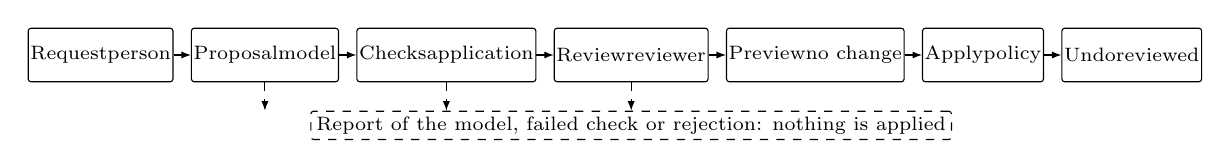
\begin{tikzpicture}[font=\scriptsize, node distance=2.2mm,
  st/.style={draw, rounded corners=1pt, align=center, minimum width=10.6mm, minimum height=6.8mm, inner sep=0.8pt},
  ar/.style={-{Latex[length=1.2mm]}}]
\node[st] (a) {\stage{Request}{person}};
\node[st, right=of a] (b) {\stage{Proposal}{model}};
\node[st, right=of b] (c) {\stage{Checks}{application}};
\node[st, right=of c] (d) {\stage{Review}{reviewer}};
\node[st, right=of d] (e) {\stage{Preview}{no change}};
\node[st, right=of e] (f) {\stage{Apply}{policy}};
\node[st, right=of f] (g) {\stage{Undo}{reviewed}};
\foreach \x/\y in {a/b,b/c,c/d,d/e,e/f,f/g} \draw[ar] (\x)--(\y);
\node[draw, dashed, rounded corners=1pt, inner sep=2pt, below=3.6mm of d] (h) {Report of the model, failed check or rejection: nothing is applied};
\draw[ar, dashed] (b.south) -- (b.south |- h.north);
\draw[ar, dashed] (c.south) -- (c.south |- h.north);
\draw[ar, dashed] (d.south) -- (h.north);
\end{tikzpicture}
\caption{Stages of the reviewed workflow and the actor of each stage. Nothing changes before Apply.}\label{fig:stages}
\end{figure}

\subsection{Architecture and scope}
Every entry point works on a declared evidence scope: the first six or ten items of the user's uncontrolled list. The interface accepts at most 20 items, and at most 12 for the staged new category. The application assesses no other item and does not search the catalogue, so a control changes at most that number of items. In the demonstration scenarios the scope is the whole invented catalogue.

A model proposes. The application checks the proposal against a schema and the supplied evidence. A reviewer, a person in the intended use, reviews the meaning and the membership. A deterministic policy, separate from the policies of Experiments 1 and 2, applies exactly the approved set. An approved boost or reduction adds or subtracts 0.10, 0.25 or 0.40 on the normalized score of each approved member, an approved exclusion removes the members, exclusion wins over an adjustment, and the item identifier breaks ties.

A proposal changes nothing: the preview shows the feed before and after, and the active state stays as it was. Apply needs the plan that the server holds for the current revision; a stale or replaced plan is refused. Undo is itself previewed and then approved, and it restores the earlier state. Each approved group is sealed with digests of the source records, the supplied items, the request and the action, and it is checked again before every use. The review screen separates the model output, the checks of the application and the decision of the reviewer, and it lists every item of the scope with the evidence for its inclusion or exclusion.

\subsection{Four entry points}\label{sec:entry}
The workflow has four entry points: a manual category control (no model call), a request matched to existing categories and tags (one call), a request matched to item descriptions (two calls) and a new category in stages (three calls). The repository records call the third the indirect request and the fourth the new category. The manual category control is the reference. The user selects an existing category and an action, and no model is called. The members are the items of that category inside the scope, so this is not the catalogue-wide category policy of Experiment 1.

\textbf{A request matched to existing categories and tags.} One model call receives the request and the list of category and tag terms that exist in the supplied items. It receives no item description. It returns one or more controls, each with an action, a verbatim part of the request and the terms that it selects. The application accepts a term only if it exists exactly in the list, and it then selects the members deterministically: the items that carry an approved term. The filter is thus the same exact-set filter as in the manual control; only the choice of terms comes from the model. A request can hold several controls, for example ``more music videos, and remove anything about food''.

\textbf{A request matched to item descriptions.} The first call interprets the action and marks the verbatim part of the request that names the subject. The second call receives the supplied items with their text fields (descriptions, tags and category names) and proposes members. For each member it must cite an exact, non-empty quotation from a named field of that item. The application rejects an unknown item, a duplicate or a quotation that is not in the field.

\textbf{A new category in stages.} The user states an objective and chooses the direction and strength. The first call receives the objective, the supplied items and the existing categories, and it proposes a label and a definition with supporting quotations. The reviewer approves or rejects the definition. The second call classifies every supplied item as match, no match or unknown. A third call assesses the evidence for every item without seeing the classification. The three calls use the same model. An item becomes a member only if the two calls agree. Every disagreement is withheld as unknown. One normalization is documented: an uncited field name of an unknown verdict is set to empty and shown in the review. The record states that semantic truth is not verified: two calls of one model can agree and both be wrong. The review screen lists every item and tells the reviewer to read each row; it cannot enforce this.

The application also keeps an earlier one-call induction, a user-confirmed target and the topic-profile path of 4 November.

\subsection{Clarification and abstention}
The workflow prefers no change to a wrong change. It abstains in two ways. First, the model can report a problem: competing interpretations, no match, or an operation that the controls cannot express, such as a quota or a time condition. The application then stops and shows the report with its alternatives. This abstention depends on the model: the application has no check that detects a quota or a condition. Second, a few fixed rules stop a request. One English pattern stops a negated control verb (``do not'', ``don't'', ``never'' or ``not to'', followed by hide, exclude, remove, reduce or boost, or by ``show'' with ``more'' or ``less'') before any model call in the two entry points that match a request (categories and tags; item descriptions). ``Do not show'' is not stopped: it goes to the model as an exclusion request. Other wordings of a negation are not detected and reach the reviewer. A selection of more than half of the supplied items also stops a request in these two entry points. For categories and tags the limit holds for each control and for the exclusions of one request together; for item descriptions it holds for the selection. The staged entry point and the manual control have no such limit. Effects that add up across requests are shown to the reviewer as notes and do not stop a request. An oversized evidence set is refused; nothing is truncated silently. When the workflow abstains, nothing is applied. A quotation shows that words are present, not that a membership decision is right.

\subsection{Model routes}
The workflow depends on one function that takes a request and a JSON schema and returns JSON. A route supplies that function. There are four: a file relay that an operator carries, a local command-line program (two profiles), an OpenAI-compatible endpoint (hosted, or a local model server) and the Anthropic Messages API. Every route follows one reply rule: exactly one JSON object, decoded strictly and validated against the schema. A route does not repair a reply and does not retry. The identity of the route and the declared model are stored with every review. A change of route changes neither the policy nor a frozen experiment: Experiments 1 and 2 stay bound to their recorded local model, and a comparison of models is a new experiment with its own protocol. A route trial tool runs the bundled requests through a route without a browser, up to the first review step. Of the four routes, only the relay has carried real model output; the other three were tested with stand-in programs and servers. Earlier direct connections remain in the code; one of them, to a command-line program, carried the runs of 10 and 11 November.

\section{Evidence Related to the Reviewed Workflow}
This evidence is separate from Experiments 1 and 2. None of it measures the accuracy of the four entry points (Section~\ref{sec:entry}). It has three kinds: a synthetic-language study of an earlier pipeline, development records and demonstration runs.

\subsection{Synthetic-language study of 4 November 2026}
The study evaluated an earlier pipeline, the reviewed topic profile of 4 November. It is not one of the four entry points. A local Qwen2.5-Coder 7B Instruct model (\url{qwen2.5-coder:7b-instruct}, Ollama 0.34.0) proposes an operation, a strength and a subject. The application grounds the subject in literal phrases of the item source text, and a deterministic policy applies the resulting profile. The requests quoted literal Chinese source phrases as their subjects, so the study tests control of a named source scope, not indirect wording. The proposed profile was scored directly; no reviewer took part. An AI author wrote 100 supported requests and 20 ambiguous or unsupported diagnostic requests, and a second AI role reviewed the locked references. The protocol was frozen before inference. Inference ran once, with no retry, and predictions were hashed before the references were opened.

The pipeline matched the complete intended profile on 48 of 100 supported requests and clarified correctly on 19 of 20 diagnostic requests. The 120 invocations gave 49 ready proposals, 61 clarifications, five grounding errors and five parser or schema rejections. Of the 52 failures on supported requests, 42 were clarifications and ten were errors. The one diagnostic failure was a proposal that the pipeline marked ready. By stratum, the correct counts are 11, 7 and 8 of 20 for single boosts, reductions and exclusions, 15 of 20 for two-topic requests, 1 of 10 for profile replacements and 6 of 10 for single subjects with context. This is a negative finding for autonomous use. The bank is now exposed.

The study also compares the intended profile (the model-written reference, applied without a model) with the profile that the model proposed, on the same 72 score vectors of 24 users and three seeds. Relative to the initial profile, the intended profile changed top-ten exposure by 5.3579 percentage points and the model-proposed profile by 2.9292 points; the direction is measured against the reference change. Both use the same policy, so the difference comes from interpretation: after a clarification or a failure the model path keeps the initial profile. HR@1 and NDCG@10 are 2.33\% and 0.0611 for the intended profile and 2.29\% and 0.0617 for the model-proposed profile, against 2.54\% and 0.0650 for the initial profile and 2.78\% and 0.0687 for the history alone. These are signed descriptive averages, not success rates, with no intervals and no tests, on reused historical relevance labels. A later project record states that the full rankings were repaired and verified separately; no record in the repository explains the repair.

\subsection{Development records}
The development records hold negative results, and they are kept. A frozen twelve-request study of 5 November gave no approved application: new category 0 of 4 supported and 1 of 2 diagnostic requests; indirect request 0 of 4 supported and 0 of 2 diagnostic requests. The six indirect cases stopped at a validation rule for the strength of an exclusion, before any item was assessed. This is a format failure, not a measured semantic accuracy of zero. The repository record does not name the models of this study. Across 14 retained development invocations on indirect requests, no local model produced an approvable item set. The first frozen development run of the staged workflow had 0 of 2 applied successes. In it, one local model proposed a definition whose quotations did not contain the claimed property. The quotations were valid, and the reviewer of that run, an AI assistant, rejected the definition. In a diagnostic with a supplied definition, the same model selected three items that the definition did not cover. These records show that the mechanical checks accept a wrong definition. Whether a human reviewer catches such an error has not been measured.

\subsection{Demonstration runs}
On 13 November 2026 (Vancouver; the receipts give UTC times on 14 November) seven runs with real model output were recorded on earlier revisions of the application, in a scripted headless browser, on two invented scenarios of eight items each with a labelled diagnostic scorer. Six runs completed. One early new-category attempt was rejected: its definition had 1,062 characters against a limit of 1,000 that the request did not state. The prompts now state the limits; schemas and validators did not change.

In each completed run the preview changed nothing, Apply removed exactly the approved items, and the two-step Undo restored the identical feed. The manual category control went from 8 eligible items to 6 and back to 8. The new category went from 8 to 5 to 8 in three runs, with the same three members from three differently worded definitions. The indirect request ``I'm not hungry, remove all the stuff that makes me hungry'' went from 8 to 5 to 8 in three runs, with the same three items and a quotation from each description. That scenario has no category or tag that names food, so those runs show a match through descriptions, not a match to a category or tag name.

The model replies came from sub-agents of one AI session through a file relay. The declared model is claude-fable-5-2; the transport cannot attest it. The same session wrote the code changes of that day, drove the browser and made every review decision. The review is therefore neither human nor independent. Its decisions took 0.5\,s to 15.5\,s (154\,s in one case), and two undo approvals were written without a reading of the undo screen. The start context of a sub-agent held the project instructions, which name a hunger-to-food example, so the model was probably not blind to the intended answer. The three runs of each entry point used three successive revisions of the application. The invented descriptions were written for these requests and state the cue in words: three say that the food is edible or to be eaten, and three say that no food is shown. In the new-category runs the objective named no concept, and the direction was chosen by hand. No automatic model connection has completed the new-category entry point: one attempt failed for an unknown cause, and a later one stopped at a clarification. The runs show that three entry points (manual category, item descriptions, new category in stages) execute from end to end on these scenarios; they are not an accuracy result. The category-and-tag entry point did not exist then.

\textbf{Runs on the final build.} The runs of \FinalRunDate{} used application revision \FinalRevision{} (source fingerprint \FinalFingerprint). Their limits are of the same kind as those of 13 November. The model replies came through the file relay from sub-agents of the AI system that also operated the review. The declared model, \FinalModel, is not attested, and the sub-agents were probably not blind to the purpose of the scenarios. An AI operator made every review decision, and no person has reviewed a run with real model output. Authored replies served the rehearsals. The command-line and HTTP routes ran against stand-in programs and servers only: no real provider, local model server or command-line program was called, and the runs were made on Linux only. The category-and-tag scenario has \FinalScenarioItems{} invented items with existing categories and tags. Table~\ref{tab:final} gives the recorded outcomes; the records are in \FinalEvidencePath. In total, \FinalAssertions. Route checks: \FinalRouteChecks.

\begin{table}[t]\centering\footnotesize
\caption{Demonstration runs on the final build (invented items, diagnostic scorer; not an accuracy result)}\label{tab:final}
\begin{tabular}{L{2.7cm}L{5.1cm}}\toprule
Flow & Recorded outcome\\\midrule
Manual category & \FinalManual\\
Categories and tags & \FinalTags\\
Mixed request & \FinalMixed\\
Ambiguous, negated, unsupported and no-match requests & \FinalAbstain\\
Item descriptions & \FinalDescriptions\\
New category in stages & \FinalNewCategory\\
Fictional item & \FinalFictional\\\bottomrule
\end{tabular}\end{table}

\subsection{Model comparison and fictional items}
A comparison of a stronger model with the local models was planned; one small record exists. In a standalone batch of six invented cases (two proposals, four abstentions), the recorded scoring reports that a Claude model matched 6 of 6 tasks and 36 of 36 item dispositions. A local Llama model and a later Qwen run failed strict JSON validation, so their semantic answers are missing; a format failure is not a measured accuracy of zero. The conditions used different transports and settings, the batch is small and exposed, and the comparison did not run through the application. The scoring archive is not in the public repository, and the record names no model version. It does not establish that one model is better than another. The route layer and its trial tool are designed to allow a like-for-like comparison; none has been run.

New items with descriptions were also planned. The application can draft metadata for a fictional item: a model writes a title, a description and a category label from a brief, a reviewer accepts or rejects the draft, and an admitted draft goes to a separate feed in which every item has score zero. It never enters the observed catalogue or the trained scorer, and its origin label cannot be changed. One run of 10 November drafted, admitted, removed and restored one item through direct calls to the application; a script made the review decisions, and the model was reached through a command-line program (reported model claude-fable-5-2). A fictional item is authored demonstration data, not a new item of the research dataset, and it gives no evidence about cold-start recommendation.

\section{Supported Claims, Limits and Reproducibility}
Table~\ref{tab:claims} separates four kinds of claim. Evidence for one kind does not transfer to another.

\begin{table}[t]\centering\footnotesize
\caption{Four kinds of claim and the evidence for each}\label{tab:claims}
\setlength{\tabcolsep}{4pt}
\begin{tabular}{L{1.6cm}L{3.75cm}L{2.5cm}}\toprule
Claim&Evidence that exists&What is missing\\\midrule
The filter applies the approved set&Enforcement in Experiments 1 and 2 (their own policies); software tests with authored replies; scripted browser checks of preview, Apply and Undo on invented items&A bit-identical replay of Experiment 1; the workflow with the trained recommender; an independent check\\
The interpretation is correct&79 of 100 (Experiment 1, authored rubric labels); 76 of 100 (Experiment 2) and 48 of 100 (4 November, earlier pipeline), both against model-written references&Any measurement of the four entry points; human references; unseen natural requests\\
Ranking quality is kept&Not kept: NDCG@10 falls for boosts in Experiment 1 and for the pooled requests of Experiment 2; it rises slightly for mutes&A meaningful margin; a stronger backbone\\
People can use it and benefit&None&A user study\\\bottomrule
\end{tabular}\end{table}

\textbf{Construct and external validity.} Requests are synthetic, and the experiment categories are opaque. There is no user study: the work observes no real steering intention and measures no comprehension or satisfaction. The next-item label is a historical proxy that a steering request can contradict. KuaiRec's platform, period, positive-event threshold and filtered cohort limit generalization, and the backbone is weak and untuned.

\textbf{References and exposure.} The references of the practice evaluation, of Experiment 2 and of the 4 November study were written by models. Shared templates limit language independence, and every bank that has been used once is exposed and cannot serve again as an unseen test.

\textbf{Demonstration.} The demonstration scenarios use invented items and a diagnostic scorer, not the trained recommender. An AI agent or a script made every review decision, and a few repeated runs on exposed scenarios are not a reliability figure. For the four entry points, the repository records on the KuaiRec catalogue show completed manual controls only; the model-based development invocations on KuaiRec text produced no approvable set.

\textbf{Reproducibility.} The protocols, compact evidence files and the application are in the repository \url{https://github.com/vibhormalik95-hue/FP}. The research archive, which is not public, holds complete cases, model responses, ranking records and checkpoints. The Experiment 2 values were checked against the public summary files. No Experiment 1 result file is in the public repository: its values are copied from the paper of 19 October 2026 and from project documents, and their primary records are in the research archive. The same holds for the twelve-request study, the fourteen development invocations, the six-case comparison and the student check. A different inference runtime may change model outputs.

\section{Conclusion}
A deterministic category policy changes exposure strongly and predictably, and it lowers next-item ranking quality for boosts. On canonical requests it shows no advantage of a language model over rules. On fresh synthetic requests with model-written references, a local model compiles compound, graded and floor requests far more often than a rule parser, fails on conditional requests, and again has a lower NDCG@10. The parser target of the proposal was missed, and useful non-inferiority was not established.

The reviewed workflow implements controls for existing categories and tags, for item descriptions and for new categories. Its interface shows each change with its evidence and offers a reviewed undo. Its evidence is of a different kind: no entry point has an accuracy measurement, a synthetic-language study of an earlier pipeline gave 48 of 100 complete profiles, development with local models failed often, and the demonstration runs show only that the steps execute on invented items with an AI reviewer. Interpretation is the open problem, and the workflow depends on a review step whose effect has not been measured. Independent human references, unseen requests, a stronger backbone and a user study are the next steps.

\bibliographystyle{IEEEtran}
\bibliography{references-2026-11-14}
\end{document}
